\documentclass[11pt]{article}
\usepackage{amssymb}
\usepackage{algpseudocode}
\usepackage{algorithm}
\usepackage{setspace}
\usepackage{graphicx}
\graphicspath{ {./images/} }
\usepackage{hyperref}
\usepackage{siunitx}

\hypersetup{
    colorlinks=true,
    linkcolor=blue,
    filecolor=magenta,      
    urlcolor=cyan,
}

\title{MSc Project - Binding Affinity Prediction of Protein-Ligand Complex}
\author{
        Abdus Salam Khazi\\
        \href{mailto:abdus.khazi@students.uni-freiburg.de}
                {abdus.khazi@students.uni-freiburg.de}\\ \\
        \href{https://github.com/abduskhazi/MSc-Project}
                {Github Repository} \cite{github_repository} \\ \\
        Supervisors:
        \begin{tabular}{ll}
			Simon Bray \&
			Alireza Khanteymoori
		\end{tabular}
       }
	
\begin{document}

\maketitle
\date{}
\tableofcontents
\newpage

\section{Introduction}

\subsection{Biological Background}
Proteins are the workhorses of our body.  They are necessary for many important functions in the body.  Ligands are molecules that bind to proteins to form protein-ligand complexes.  They can be molecules that the protein transports (e.g., a Haemoglobin transporter) or act as stimulating agents.  In addition to this, they can also start/stop the protein from doing its function.  The correct functioning of these protein-ligand complexes is essential for any living organism.

The study of protein-ligand complexes is an intrinsic part of the drug discovery field.  It is because drugs are small molecules that act as ligands.  As the drug molecules (ligands) bind to the target proteins, they can artificially influence the protein behavior.  This causes a therapeutic effect.

\begin{figure}[htb]
  \centering
    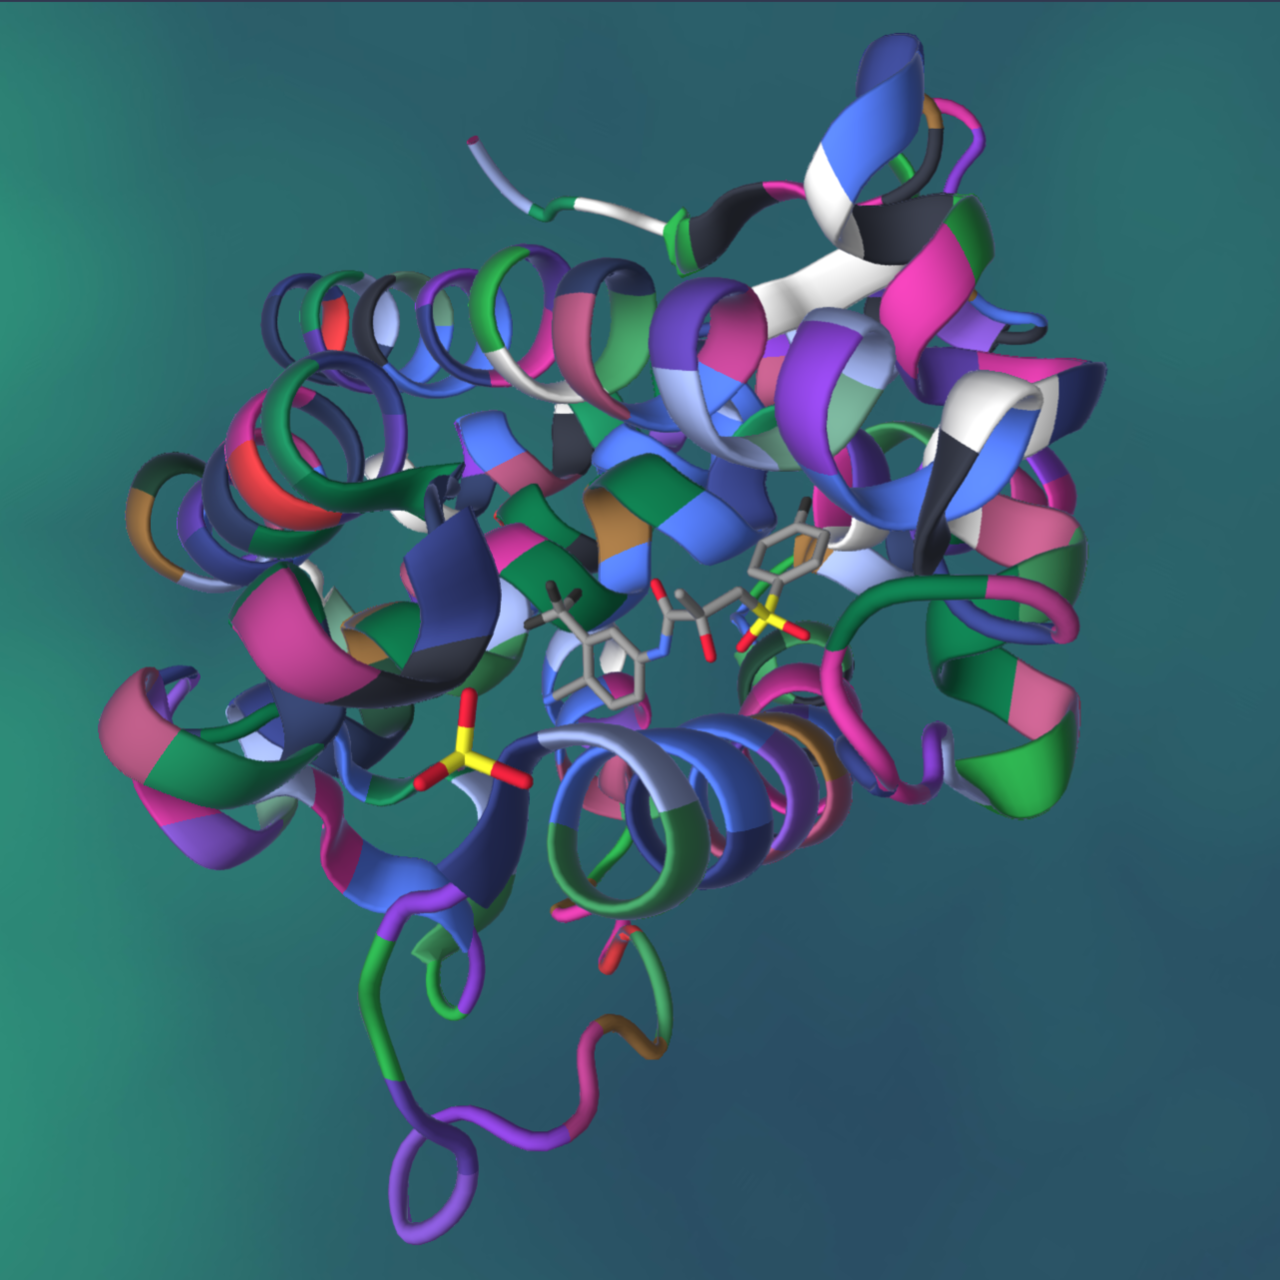
\includegraphics[scale=0.15]{images/pl_complex}
    \caption{Haemoglobin transporter protein.  \cite{PL_complex_introduction}}
    \label{fig:HaemoglobinTransporterImage}
\end{figure}


When we find a target drug candidate, we have to answer questions like - How easily does the drug bind to the target protein? Does it bind to any other protein - If so, is it desirable? Does it have any unforeseen effect on the protein function? etc...  To answer these questions biologists and pharmacists conduct wet-lab experiments that are expensive.

One way to reduce the cost of these experiments is to make a data-driven selection of the drugs.  Using experimental data collected over many years, one can build models to predict the behavior of the proposed drug computationally.  These 'In-Silico' computational methods can aid in the elimination of undesirable drugs as well as guide the drug selection process.

Our project aims to answer one of the above questions - How well does a given drug bind to the target protein? We determine this computationally by building a machine learning model that trains on the previous data.  We hope that this model will help reduce the costs of drug discovery.  But from where do we get the data to build our model?

\subsection{PDBBind Dataset}
Over the last few decades, researchers have been successful in building a single data archive for proteins.  This archive, called \textbf{Protein Data bank} \cite{pdb_homepage} , holds 3-D structural data of the proteins determined by experiments like X-ray crystallographic, Nuclear magnetic resonance (NMR), and cryoelectron microscopy (cryoEM).  A subset of this data also contains information about how well a given protein and ligand bind together.  It is called binding affinity between a protein and ligands.  (It also contains data about protein-protein complexes that our project does not deal with)
\cite{pdbank_history}

As we study the protein-ligand binding affinity here, we would like to filter out this data from the protein data bank.  It is what is done by the maintainers of the \textbf{PDBBind Data bank}.
\cite{pdbbind_introduction}
Using the curated protein-ligand affinity data present in the PDBBind Data bank, we build a machine learning model that learns to predict the affinity.  But how is the binding affinity quantified?

\subsection{Understanding Binding Affinity}
The binding affinity between a protein and a ligand is quantified by the $K_d$, $K_i$ and $IC_{50}$ measures in the PDBBind Data bank.
Here $K_d$ refers to disassociation constant, $K_i$ refers to the inhibition constant, and $IC_{50}$ refers to 
inhibitory concentration 50\%.
The reason for having different measurements is because it is not possible to use the same measurement techniques
for all biological complexes/processes.

To understand $K_d$, consider a protein and a ligand binding and unbinding continuously in a kinetic system.
In this system, let $[P]$, $[L]$, and $[PL]$ represent the concentrations of the Protein, the Ligand, and the Protein-Ligand complex respectively.
This is represented by the following equation:
$$[P] + [L] \rightleftharpoons [PL]$$
We can quantify the binding affinity $K_d$ by using the concentrations in the above system at equilibrium.
$$K_d = \frac{[P][L]}{[PL]} = \frac{k_{-1}}{k_1}$$
where $k_{-1}$ is the disassociation rate constant and $k_1$ is the association rate constant.
Similarly, $K_i$ and $IC_{50}$ are defined using concentration albeit non-trivially. 
\cite{binding_affinity_description}

Our problem, hence, boils down to this - Given $K_d$/$K_i$/$IC_{50}$ for various complexes in the PDBBind Data bank,
can we predict this affinity measure for new protein-ligand complexes?

The next questions that need to be addressed before we build our agent are - how exactly are the proteins and ligands represented in the PDBBind Data bank?
How do we extract the properties of proteins and ligands for predicting this affinity?

\section{Problem Set-up and Formulation}

The binding of proteins and ligands is heavily influenced by their respective 3D structures.
The \textbf{PDBBind Data bank} extracts information about these complexes from the \textbf{Protein Data bank} and creates the following files for every complex
\begin{itemize}
\item \textbf{PDB Format} - For the Protein.
\item  \textbf{Mol2} - For the ligand.
\item \textbf{SDF} - For the ligand.
\end{itemize}

All of the above formats contain 3D information that is essential in the prediction of the binding affinity.
The 3D representation of the proteins and ligands is similar to the \textbf{XYZ format}.
[See \ref{xyz_format}]

\subsection{Overview of file formats}
\subsubsection{XYZ format}
\label{xyz_format}
XYZ format is a chemical file format that represents the geometry of a molecule.
It specifies the number of atoms and their Cartesian X, Y, Z coordinates hence the name XYZ format.
The coordinates are relative to each other. Hence, translation and rotation do not change the molecule's representation. 
The following text illustrates the XYZ format.
Section \ref{XYZFileexampleref} gives an example.
\cite{XYZ_format}
\begin{verbatim}
<number of atoms>
comment line
<element> <X> <Y> <Z>
...
\end{verbatim}

The unit of distance used is Angstrom (\si{\angstrom}).  \SI{1}{\angstrom} $ = 10^{-10}$ m.
\cite{XYZ_format}

\subsubsection{PDB format}
PDB format is a human-readable file format used to represent the protein molecules (macromolecules).
Within the PDB format,  the coordinates of atoms are represented like the XYZ format [see \ref{xyz_format}].
Because of the 3D information in this format,  molecular visualization of proteins is possible with specialized software. 
It also contains information about atomic connectivity and the protein's primary,  secondary,  tertiary,  and quaternary structures.
\cite{pdb_file_format}
\cite{understanding_pdb_format}
Please see \cite{examplePDBFile} for an example pdb file.


\subsubsection{Structure Data File (SDF) Format}
SDF format file is a Chemical Table file (CT File) that contains structure of the molecule in the X,Y,Z format.
It contains information like atomic bonds,  connectivity information,  molecular weight,  and molecular formula. \cite{SDFformat}
Section \ref{SDFFileexampleref} illustrates the SDF file format.

\subsubsection{Mol2 format}
Similar to SDF format,  Mol2 also represents the 3D structure of a molecule in the X,Y,Z format.
It contains the atomic bond and connectivity information but does not contain the other data like molecular weight and formula.
We use the ligands given in this format because more ligands in mol2 format could be processed with the RDKit feature extractor.
Section \ref{MOL2Fileexampleref} illustrates the Mol2 file format.

\subsubsection{SMILES format}
SMILES is an acronym for Simplified Molecular-Input Line-Entry System.
It represents a molecule using an ASCII string.
Using the 3D data in SDF and Mol2 formats,  we can create an atomic graph representation.
Using this graph the SMILES string for the molecule can be generated.
The smiles format itself is not very helpful for us as we lose the 3D structural information after converting to it.
\cite{smilesformat}

\subsection{Problem Formulation}
Protein-Ligand complex problems are classified into two types -
\begin{itemize}
\item LBS - Ligand binding site prediction.
\item Ligand affinity prediction.
\end{itemize} 

LBS (Ligand binding side) prediction can be further classified into 3 types -
\begin{itemize}
\item 3D structure based
\item Template based
\item Sequence based
\end{itemize}

We deal with binding affinity prediction in our project.
In our problem, we take care of the following two things
\begin{itemize}
\item We take the features of the pocket in the protein structure that binds to the ligand. It is the site where the ligand is bound to the protein, just like a key is attaching to a lock.
\item To get a plug-and-play input to our model, we keep the features of proteins and ligands distinct till the input step.
It helps our model to provide the binding affinity between any protein and ligand.
\end{itemize}

However, for this, we make use of the existing 3D structure-based LBS toolchain called fpocket.
It is because 3D structural features of proteins are very crucial for protein-ligand binding. The Proteins-Ligand interactions can be seen as two parts of a machine interacting with each other.

\subsection{Extraction of features}
\subsubsection{Ligand Featuers using RDKit}
\subsubsection{Protein Features using fpocket/dpocket descriptors}
We extract the features of a pocket using dpocket tool (a submodule in the fpocket toolchain).
fpocket uses voronoi tessalation (3D) to find out pockets in our protein structure.
To get the descriptors/features of the pockets at which ligands bind we use the dpocket (aka descriptors pocket).
dpocket creates 3 types of descriptors for the pockets in the protein -
\begin{itemize}
\item fpocketp.  This lists all the possible pockets (with descriptors) that could bind to ligand according to a criteria.
Multiple pockets can bind with the same ligand.
Here the descriptor called overlap maybe 100\% or less.
\item fpocketnp.  This lists all pockets (with descriptors) that are not binding according to the criteria.
\item explicitp.
This lists all the explicitly binding pocket (with descriptors).
Here the overlap feature is always 100\%.
\end{itemize}

We use both fpocketp and explicitp descriptors to train our model.
There are in total 55 descriptors in total obtained using dpocket descriptors.



\section{Feature selection}

\subsection{Dichotomous problem}
Since the protein and the ligand are equally responsible for the affinity between them, our problem (also the binding site prediction problems) can be classified as a dichotomous problem in which we need data from both
the protein and the ligand.
The data if it is complementary is better for solving the problem.
The accuracy measure of the protein LBS prediction is the same as the dichotomous problems in math.

As we are dealing with a dichotomous problem we have to select features of the protein and the ligand separately.
This helps us make our model plug and play w.r.t the proteins and ligands.
The following feature selection mechanisms were used to select features -

\begin{itemize}
\item Each feature of both protein and ligand were correlated with the output i.e the Dissociation constant.
We used both pearson and spearmann correlation to calculate this.
The assumption to be made when taking these correlations is that of monotonic increase of
the feature with respect to the output.
The features with the highest correlation were taken from both proteins and ligands as
inputs.
\item By using genetic algorithms\cite{genetic_algorithm}.
Here each feature is represented by a binary number.
1 indicating inclusion and 0 indicating exclusion from the input of our model.
A binary string of 456 binary numbers (401 for ligands + 55 for proteins) is called a chromosome.
See pseudocode below
\item Features selected by expert. Given by Simon Bray. (Yet to do)
\end{itemize}

\label{Genetic_Algo}
\begin{algorithm}
\caption{Selection of features in our model using genetic algorithm \cite{genetic_algorithm}}
\begin{algorithmic}[1]
\Procedure{GENETIC\_ALGORITHM\_BASED\_SELECTOR}{}
\State model\_type $\gets$ Linear Regression
\State $ population = \{C_1, C_2, C_3... C_n\}$ $\in$ $\mathbb{B}^{456}$ (initial chromosomes).
\State best $\gets C_1$ 
\State $i \gets 0$
\State $gen \gets$ number of generations to run.
      \For{\texttt{$i < gen$}}
          \State Fit model\_type for each feature selection (chromosome). 
          \State Let $\{S_1, S_2, S_3... S_n\}$ $\in$ $\mathbb{R}$ be scores for each chromosome.
          \State best $\gets$ $C_i$ with the highest score $S_i$
          \For{\texttt{$j < len(population)$}}
              \State Set $\gets$ 3 random chromosomes from $population$
              \State $c \gets best($Set$)$
              \State $genetically\_better\_population.add(c)$
          \EndFor
          \State $population \gets genetically\_better\_population$
          \For{\texttt{$j < len(population)$ with step 2}}
              \State $P_1, P_2$ $\gets$ $population[j], population[j+1]$
              \State $c_1, c_2 \gets crossover(P_1, P_2)$
              \State $c_1 \gets mutation(c_1)$
              \State $c_2 \gets mutation(c_2)$
              \State $children.add(c_1, c_2)$
          \EndFor
      \State $new\_population \gets population$
      \EndFor
\State return best
\EndProcedure
\end{algorithmic}
\end{algorithm}

\section{Testing}
\subsection{Reproducibility}
Reproducible ML models are very crucial for verifying any project or research results. Due to the stochastic nature of many ML training processes, reproducing the exact model (and consequently the exact output) is a challenge. Two methods can be employed to produce verifiable results:
\begin{itemize}
\item Training many models and reporting the average results.
\item Controlling the randomness of the trained models. It is done by setting the seed of the pseudo-random algorithms.
\end{itemize}

We use the second approach in our project. Every script, when executed, reports an execution ID. This is the random seed used during the execution. If we want to reproduce the exact results, we give this execution ID to the script as the first argument.

\subsection{Model Quality Analysis}
We are trying to predict the following function
$$ \textrm{Binding affinity prediction} : \mathbf{R}^n \mapsto \mathbf{R} \;\; \textrm{where} \;\; n \in \mathbf{I}^+$$
Since the input space is multi-dimensional, we cannot fully visualize our model as a function of the input space.
To get around this using the following methods
\begin{itemize}
\item We report \textit{Coefficient of determination}, $R^2  \in (- \infty, 1.0]$ where $1.0$ is the best score. \cite{r_squared_score}
$$R^2(y, \hat{y}) = 1 - \frac{\sum_{i=1}^{n} (y_i - \hat{y}_i)^2}{\sum_{i=1}^{n} (y_i - \bar{y})^2} \;\; \textrm{where} \;\; \bar{y} = \frac{1}{n} \sum_{i=1}^{n} y_i \;\;
\textrm{and} \;\; \sum_{i=1}^{n} (y_i - \hat{y}_i)^2 = \sum_{i=1}^{n} \epsilon_i^2$$

\item For visualizing the results,  we plot a 2D plot of expected values against the output given by the model.  A perfect model would have all the points in the graph on the $y = x$ line.  This corresponds to $R^2$ score of $1.0$
\end{itemize}

Figure~\ref{fig:modelQualityVisualization},  shows the validation accuracy of \textit{Random Forest Regressor} model.

\begin{figure}[htb]
  \centering
    \includegraphics[width=1.0\textwidth]{images/accuracy_validate}
    \caption{Validation Accuracy.  $R^2 \approx 0.805$.}
    \label{fig:modelQualityVisualization}
\end{figure}

%\includegraphics[scale=0.7]{accuracy_validate}
%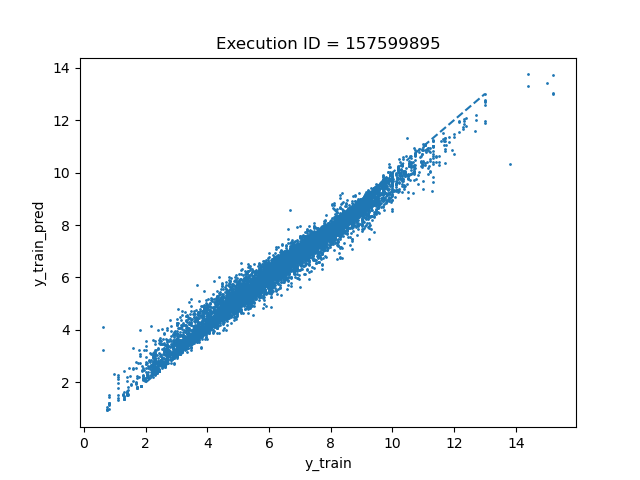
\includegraphics[scale=0.7]{accuracy_train}

\section{Machine Learning Models}

Various machine learning models were trained using the extracted data.
We tried out Linear Regression,
Support Vector Regression,
A small Neural Network,
as well as a Random Forest Regression.
But far the most impressive performance was given by Random Forest Regression.

\subsection{Simple linear regression}
This is the most computationally cheap model that we used to fit our model.
The $R^2$ score for this model we got $\approx 0.455$ when we used all the
features of the ligands and the proteins.
Since the fitting of the model was very cheap, we tried to use the validation
score of the model as a fitness score for our genetic algorithm.


\subsection{Random Forest Regression}
A random forest regression is an ensemble model which uses an ensemble of trees
to calculate the output variable.
Each node in the tree reduces tries to reduce the entropy of the data at hand.
The $R^2$ score we got was $> 0.75$ for an ensemble of $100$ trees.

\subsubsection{Feature Importance calculation}
The Random Forest regression model fitting is very expensive as compared to the simple linear regression.
Hence the same strategy cannot be used for feature selection as used in the linear models.
We used 2 main methods to determine the importance of features in the model
\begin{itemize}
\item \textbf{Gini Importance} - This is given by default by the model. The model 
calculates the amount of entropy reduction of that each feature does when it divides the data using the OOB score. (Out of bag Score)
\item \textbf{Permutation Importance} - This is a model agnostic method to determine the importance of features in a regression. 
It tries to calculate the reduction in the accuracy we shuffle each column.
\end{itemize}
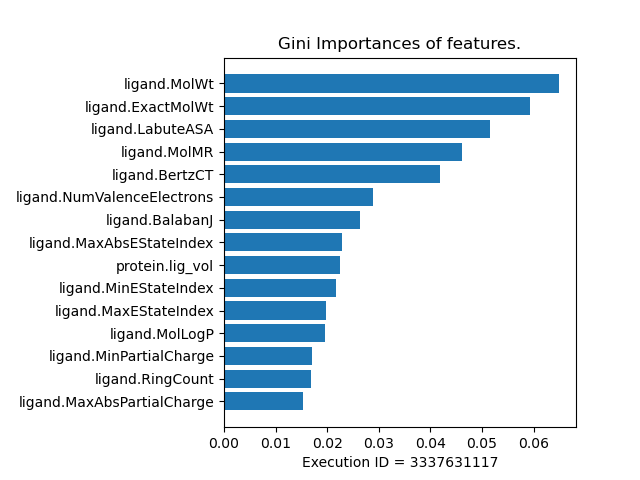
\includegraphics[scale=0.7]{Gini_importance}

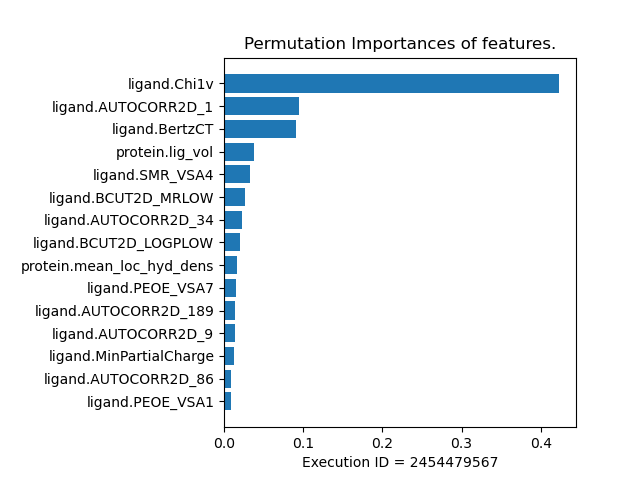
\includegraphics[scale=0.7]{Permutation_importance}

The issue with the above methods is that if there is any hidden correlation between input features then it will reduce the importance of the correlated features.

\subsection{Permutation Importance and genetic algorithm}
To overcome the issue with the above feature importance selection, we plan to use a combination of the concepts of permutation importance and genetic algorithm to find out the importance of the selected features.

Results - YET TO IMPLEMENT

\section{Discussion}


\section{Conclusion}

\bibliographystyle{plain}
\bibliography{references}

\section{Appendix}
\subsection{XYZ File format}
\label{XYZFileexampleref}
The following represents the pyridine molecule in the XYZ format.
\begin{verbatim}
11

C       -0.180226841      0.360945118     -1.120304970
C       -0.180226841      1.559292118     -0.407860970
C       -0.180226841      1.503191118      0.986935030
N       -0.180226841      0.360945118      1.29018350
C       -0.180226841     -0.781300882      0.986935030
C       -0.180226841     -0.837401882     -0.407860970
H       -0.180226841      0.360945118     -2.206546970
H       -0.180226841      2.517950118     -0.917077970
H       -0.180226841      2.421289118      1.572099030
H       -0.180226841     -1.699398882      1.572099030
H       -0.180226841     -1.796059882     -0.917077970
\end{verbatim}

\subsection{SDF File format}
\label{SDFFileexampleref}
\begin{verbatim}
2uzn_ligand

Created by X-TOOL on Fri Nov 18 14:55:27 2016
 37 39  0  0  0  0  0  0  0  0999 V2000
    7.1480   60.4530    6.6830  O 0  0  0  1  0  1
    6.0470   60.1670    7.5640  S 0  0  0  1  0  4
    .......
    .......
   -2.6338   67.4589    8.1225  H 0  0  0  1  0  1
  1  2  2  0  0  2
  2  3  2  0  0  2
  .......
  .......
 23 37  1  0  0  2
M  END
> <MOLECULAR_FORMULA>
C15H13N3O4S2

> <MOLECULAR_WEIGHT>
363.3

> <NUM_HB_ATOMS>
7  

> <NUM_ROTOR>
1  

> <XLOGP2>
1.31 
\end{verbatim}

\subsection{MOL2 File Format}
\label{MOL2Fileexampleref}
\begin{verbatim}
### 
### Created by X-TOOL on Fri Sep 26 17:34:18 2014
### 

@<TRIPOS>MOLECULE
1fo2_ligand
   25    25     1     0     0
SMALL
GAST_HUCK


@<TRIPOS>ATOM
      1 C4         39.0090   40.2680   25.5130 C.3       1 DMJ         0.1280
      2 O4         39.2170   40.5810   26.8980 O.3       1 DMJ        -0.3835
     .......
     25 H14        38.0787   41.8134   21.3802 H         1 DMJ         0.2097
@<TRIPOS>BOND
     1    1    9 1  
     2    1    3 1  
    .......
    25   11   25 1  
@<TRIPOS>SUBSTRUCTURE
     1 DMJ         1
\end{verbatim}

\end{document}
